\documentclass[12pt,twoside,norsk,onecolumn]{article}
\usepackage{a4}
\usepackage[utf8]{inputenc}  % Use latin-1 character set for input
\usepackage[norsk]{babel}    % Use English hyphenation
\usepackage[dvips]{epsfig}     % To include PostScript
\usepackage[parfill]{parskip} % New line instead of tab for paragraphs
\usepackage{nomencl}
\usepackage[firstpage]{draftwatermark}
\usepackage{url}
\usepackage{amsmath}
\usepackage{color}
\usepackage{longtable}
\usepackage{graphicx}
\usepackage{verbatim}

\renewcommand{\nomname}{Forkortelser}
\makenomenclature

\begin{document}

\newcommand{\versjon}{v0.2.1}

%Forside
\thispagestyle{empty}
\begin{center}        % Sentrerer teksten
  %Tittel
  \vspace{5mm}          % Vertikalt mellomrom
  \LARGE
  \textbf{Automatisk Planlegging i Oljeindustrien} \\
  \Large
  \vspace{5mm}
  \textbf{av} \\
  \vspace{5mm}
  %Forfatter
  \large
  \textbf{Teis Lindemark} \\
  \colorbox{red}{\versjon} \\
  %Avdeling for mekanikk
  \vspace{30mm}
  \Large
  {\bf{\textsl{AVHANDLING}}} \\
  \textsl{for en grad av} \\
  \vspace{2mm}
  %%%%%%%OLD%%%%%%{\bf{\textsl{CANDIDATUS SCIENTIARUM}}} \\
  {\bf{\textsl{MASTER I INFORMATIKK}}} \\
  \vspace{5mm}
  {\large \textsl {Masteroppgave, Institutt for informatikk}}\\
  \vspace{10mm}
  \centerline{
\includegraphics[width=4cm,height=4cm]{uibugle}}
  \vspace{5mm}
  % \textsl{Mechanics Division, Department of Mathematics} \\
  %\textsl{Fakultetet for teknologi og realfag} \\
  \textsl{Universitetet i Bergen} \\
  %Maaned, aar
  \vspace{10mm}
  \large
  \textsl{Juni 2012} \\
  \vspace{5mm}
  \normalsize
  % \textsl{Avdeling for mekanikk, Matematisk institutt} \\
  %\textsl{Fakultetet for teknologi og realfag} \\
  \textsl{Universitetet i Bergen} \\
\end{center}
% START OF DOCUMENT
\newpage
\vspace*{\fill}
%Abstract
\begin{abstract}
TEST
\end{abstract}
\vspace*{\fill}
\newpage

%Defining commands
\newcommand{\bht}{Bård Henning Tvedt }
\newcommand{\bhtmb}{Bård Henning Tvedt og Marc Bezem }
\newcommand{\ilog}{ILOG Scheduler }

%Table of contents
\tableofcontents
\newpage

%Preface
\section*{Forord}
%Først ønsker jeg å takke min instituttveileder, professor Marc Bezem, og min veileder hos Epsis, Bård Henning Tvedt for veldig god veiledning gjennom hele prosessen av dette arbeidet. Takk til at dere brukte av deres dyrebare tid for å veilede meg gjennom denne oppgaven.

Ellers må jeg også takke mine foreldre for god støtte gjennom mastergraden, som har støttet meg gjennom gode og mindre gode tider. Når jeg ikke så enden på tunnelen, var det alltid godt å kunne pratet ut og fått nødvenndig støtte. Tilslutt må jeg også takke foreldrene mine for at de kunne hjelpe til med å korrekturlese oppgaven.

Teis Lindemark, 6. Mai 2012
\newpage

\begin{center}
\printnomenclature[2.5 cm]
\end{center}
\newpage

%Introduction
\section{Introduksjon}
Denne oppgaven er en utvidelse av \bht sitt arbeid med "Automatisk Planlegging i Oljeindustrien (APO)"\nomenclature{APO}{Automatisk Planlegging i Oljeindustrien} \cite{tvedtbezem}. APO er et planleggingsproblem i industrien og det blir brukt en fiktiv platform for å kunne gjøre problemet så likt som mulig virkeligheten. Implementjonen i IBM ILOG Scheduler er utvidet med ressurser på varmebegrensning. Med varme er det ikke varme i tradisjonell forstand, men et mål for hvor mye kapasitet en ressurs bruker.

\subsection{Beskrivelse av kommende kapitler}
I kapittelet om metode, vil fremgangsmåten for prosjektet bli lagt frem og hvordan løsningene har blitt evaluert. I kapittelet om eksperimenteringen vil det legges frem løsninger ved forskjellige strategier og med og uten ressursene. Her vil også løsningene bli evaluert og tilslutt vil det bli sammenfattet en konklusjon over det arbeidet som er gjort.
\subsection{Bakgrunn}
I dette prosjektet, verktøyene som er brukt for å utføre eksperimenter på emnet er Scheduler som er endel av IBM sitt ILOG CP produkt\nomenclature{CP}{Begrensningsprogrammering (engelsk: Constraint programming)}. Scheduler er et C++ bibliotek som gjør det mulig å definere planleggingsbegrensninger i form av ressurser og aktiviteter. Planlegging er en prosess hvor det tildeles ressurser til aktiviteter og tid til de forskjellige aktiviteter slik at det ikke oppstår noen konflikt med begrensningene \cite{Pape94implementationof}. Automatisk planlegging er endel av det som kalles kunstig intelligens (AI) \nomenclature{AI}{Kunstig intelligens (engelsk: artificial inteligence)}.

I kompleksitetsteori \cite{compcomplextheory} kaller man problemer som er minst like vanskelige å løse som de vanskeligste problemene i kategorien \textit{NP} som \textit{NP-hard}. NP er kategorien av problemer som kan løses i polynomisk tid på en ikke-detministisk Turing  maskin. Det er forskjellige kategorier av NP-harde problemer, avgjøreksesproblemer, søkeproblemer og optimaliseringsproblemer \cite{nphardwikipedia}. Problemet i dette prosjektet er i kategorien optimaliseringsproblem. Fra wikipedia \cite{optimizationproblemwiki} er et optimaliseringsproblem: ''Et problem med å finne den beste løsningen ut ifra alle gyldige løsninger".

Taillard \cite{Taillard1993278} har sett på benchmarking i enkle planleggingsproblemer og sett på hvordan man best mulig benchmarker vanskelige problemer. De har definert vanskelige problemer ved å se på makespan og hvor langt unna den er den nedre grensen. De har tatt utgangspunkt i tre kjente begrensningsproblemer og laget benchmarksett til disse. Taillard har definert nedregrensen i ''Job Shop Scheduling Problem (JSSP)" som større enn eller lik maksimale mellom den minste tiden krevd av maskinene og den minste tiden krevd av hver enkel jobb. Wallace \cite{Wallace:2004:BCL:956860.956861} har også sett på benchmarking og tatt for seg positive og negative sider ved benchmarking. Benchmarking har to hovedoppgaver, hvor det første er å dekke et representativt problem og bredt programmeringsbegrep. Den andre oppgaven er benchmarking av applikasjoner med ''enhetstester". Utfordringen med begge er å opprette en klar målsetting for ytelsen. Teoretisk sett er den mest ideele måten å benchmarke en applikasjon å implementere en løsning for hvert system og velge den beste, men dette er ikke alltid mulig i praksis. Måten da å gjøre det på i praksis er å benchmarke systemer med forhåndsdefinerte problemer og håpe resultatet kan bli overført til applikasjonen som krever det. Wallace tar også opp vanskeligheten med tidsmekanismer i høynivåspråk, da dette ofte er basert på CPU tid.

%Motivasjon
\section{Motivasjon}
\subsection{Motivasjon}
Forskningen er motivert av praktisk erfaring at planleggingsproblemer er veldig aktuelt i bedrifter og i samfunnet idag. Det er ikke bare i oljeindustrien som jeg fokuserer oppgaven på hvor planleggingsløsninger er aktuelt, men generelt bemmaningsproblematikken som alle personalavdelinger sitter med i det daglige. I hverdagen er det også mange planleggingsproblemer fra buss- og togtabeller til personlige gjøremål med å få tid til alt man skal ha tid til.

Planlegging i oljeindustrien er viktig for å på en mest mulig effektiv måte benytte seg av de ressursene som er tilgjengelig til enhver tid, samtidig som visse begrensinger blir fastsatt med tanke på sikkerheten. Det er mye penger involvert i olje- og gassindustrien og det å utføre aktiviteter på en ineffektiv måte kan koste selskapene veldig mye penger. Det er derfor viktig å ha gode løsninger for å ta seg av planleggingen av aktivitetene og ressursene. Operatører innen olje- og gassektorens mål er å minimere antallet farlige situasjoner, minimere miljømessige skade og maksimere produksjon. Det å imøtekomme disse kompliserte og utfordrende målene, kan det i enkelte situasjoner oppstå konflikter.

Spesifikke planleggingssituasjoner har forskjellige forutsetninger i forhold til om plattformen er offshore eller på land. Offshore kan mange aktiviteter bli utført på et relativt lite lukket område, mens områder på land kan ha mange aktiviteter utført på et relativt stort område. Selvom forutsetningene for disse to typene plattformer er ganske forskjellige, så har de flere likhetstrekk som:
\begin{itemize}
\item størrelse - antall aktiviteter kan være noen hunder til titusener, for å gjøre planleggingen interaktiv.
\item kompleksitet - et stort antall av begrensningene som skal bli gjennomført, gjør en mulig planlegging vanskelig.
\item dynamikk - avhengigheter som vær, logistikk og utstyr som feiler kan avbryte planleggingen.
\end{itemize}

\subsubsection{Kort om begrensningsprogrammering}
Begrensningsprogrammering er en programmeringsparadigme hvor relasjoner mellom variable blir satt i form av begrensninger. Begrensninger er en form for deklarativ programmering, som skiller seg fra den mer vanlige imperativ programmeringsspråk\footnote{Imperativ programmeringsspråk har sekvenser med som blir utført.} ved at løsningen blir til ved å tilfredsstille begrensningene. Det er forskjellige områder i begrensningsprogrammering som "Constraint Satisfaction problems" og planleggingsproblemer. Det mest kjente planleggingsproblemet er "Job Shop Scheduling".\cite{cpwikipedia}

\subsubsection{Utfordringer med begrensningsprogrammering}
\colorbox{red}{Utfordringer med CP}
\begin{itemize}
\item Ytelse - begrensings logikk programmerings system ytelse mindre enn tradisjonelle imperative.
\item Ytelse - automatisk paralissering
\item Debugging og visualisering
Begrensningsprogrammeringssystemer har ofte en svakhet når det kommer til feilsøking (engelsk: debugging). Uten tilstrekkelige måter å kunne være sikkert på riktigheten og muligheter å sjekke ytelse i programmer. En måte å løse utfordringene med manglende feilsøkingsmuligheter er å bruke påstander \nomenclature{Påstander}{Engelsk: Assertions}. Ved bruk av påstander kan det opprettes post- og preforhold. Påstander kan bli sjekket ved kompilering eller når programmet kjører. Det er også mulig å genere påstander av kompilatoren, som utvikleren kan sjekke om det eksisterer høynivåfeil\cite{challengesManuel}.
\end{itemize}

\subsubsection{Begrensingsprogrammeringsverktøy idag}
Det finnes idag flere forskjellige verktøy for begrensningsprogrammering, både i form av egne programmeringsspråk som er skreddersydd for begrensningsprogrammering og biblioteker til godt kjente programmeringsspråk som Java og C++. I begge disse kategoriene så finnes det løsninger som er kommersielle og med åpen kildekode. Noen eksempler på egne programmeringsspråk for begrensningsprogrammering er Prolog og Comet. Sistnevnte er et programmeringspråk for begrensningsprogrammering med lokalt søk og er en kommersiell løsning. Eksempler på begrensningsprogrammeringsbiblotek så er det IBM ILOG CP.

Planlegging er ofte tett knyttet opp mot prosjektstyring og prosjektstyringsverktøy finnes det veldig mange av etterhvert \cite{projectmanagmenttoolswiki}. Både programmer du har lokalt på maskinen og også webbaserte tjenester. Fellesnevneren for veldig mange av disse tjeneste, enten de er lokalt eller webbaserte er at de skal hjelpe til med alt fra prosjektplanlegging, dokumentdeling, oversikt over oppgaver, oversikt over frister, møteplanlegging og mye mer. Denne typen programvare er ofte gjort ganske enkle å bruke, men det er noen programmer som gjør det mulig å definere aktiviteter (eller oppgaver) og knytte ressurser til aktivitetene. Et eksempel på et slikt program er Microsoft Project. Dette programmet har et grafisk grensesnitt som andre programmer i Office-pakken til Microsoft og er et enkelt program å bruke. Microsoft Project 2010\nomenclature{MSProject}{Microsoft Project 2010} gir muligheter til manuell og automatisk planlegging\cite{msproject2010blog}. I MSProject er det mulig å legge til begrensninger, men ser ganske begrenset ut til aktiviteters starttidspunkt\cite{begrensingermsproject}.

Det finnes få verktøy for å gjøre begrensingprogrammering som er kan brukes rett ut av boksen idag, enten det er logisk problemløsning eller planleggingsløsning. Noen verktøy er bedre på logisk problemløsning og andre på planleggingsproblemer. Det finnes også mange forskjellige problemmer innen begge kategorier som er komplekse og det er derfor nødvenndig å finne verktøyet som passer best mulig til problemet som skal løses. Innen industrien er det ofte ressurser som stiller krav utover standardiserte problemer.

\subsubsection{Forbedringerspotensiale i verktøyene}

\subsubsection{Relevans for forskingen}

%Problemstilling
\section{Problemstilling}
\subsection{Problembeskrivelse}
Hvordan påvirker ekstra ressureser og begrensinger løsningene i ILOG?

Tester paragraf.

%Begrensning
\section{Begrensning}
I denne delen blir det gitt en innføring om begrensningsprogrammering og utfordringer som kommer med begrensningsprogrammering. Det vil også bli sett litt på verktøy som eksisterer idag for å bruke begrensningsprogrammering samt noen enkle verktøy for enkel planlegging av aktiviteter og ressurser. Tilslutt i denne delen er det en kort beskrivelse av verktøyene som er brukt i dette prosjektet.

\subsection{Kort om begrensningsprogrammering}
Begrensningsprogrammering er en programmeringsparadigme hvor relasjoner mellom variable blir satt i form av begrensninger. Begrensninger er en form for deklarativ programmering, som skiller seg fra den mer vanlige imperativ programmeringsspråk\footnote{Imperativ programmeringsspråk har sekvenser med instanser som blir utført.} ved at løsningen blir til ved å tilfredsstille begrensningene. Det er forskjellige områder i begrensningsprogrammering som ''Constraint Satisfaction problems" og planleggingsproblemer. Det mest kjente planleggingsproblemet er ''Job Shop Scheduling" \cite{cpwikipedia}.

\subsection{Utfordringer med begrensningsprogrammering}
Systemer for begrensings-logikk programmeringssystemer som sammenliggnes med begrensningsløsningssystemer, er ofte ytelsen bedre i begrensings-logikk programmeringssystemer. Ytelsen er likevel ikke like god som mer tradisjonelle imperative programmeringsspråk, og spesielt gjelder det innen tallmessige utregninger. For å løse dette, er det mulig å utvikle en avansert kompilator som sjekker de tilfellene hvor det ikke er behov for begrensingsløning, og da kompilerer disse på mest mulig effektive måte \cite{challengesManuel}

Begrensningsprogrammeringssystemer har ofte en svakhet når det kommer til feilsøking (engelsk: debugging). Uten tilstrekkelige måter å kunne være sikkert på riktigheten og muligheter å sjekke ytelse i programmer. En måte å løse utfordringene med manglende feilsøkingsmuligheter er å bruke påstander \nomenclature{Påstander}{Engelsk: Assertions}. Ved bruk av påstander kan det opprettes pre- og postforhold. Preforhold skal resultere i en boolsk verdi (sann eller falsk) og metoden blir ikke utført hvis ikke preforholdet er sant. Postforhold til en metode beskriver hva som skal være oppnåd med metoden. Postforold er også en boolsk verdi. Både pre- og postforhold blir skrevet for å ''evaluere" en metode, enten før metoden blir utført eller hva metoden har oppnåd. Påstander kan bli sjekket ved kompilering eller når programmet kjører. Det er også mulig å genere påstander av kompilatoren, som utvikleren kan sjekke om det eksisterer høynivåfeil \cite{challengesManuel}.

\subsection{Begrensingsprogrammeringsverktøy idag}
Det finnes idag flere forskjellige verktøy for begrensningsprogrammering, både i form av egne programmeringsspråk som er skreddersydd for begrensningsprogrammering og biblioteker til godt kjente programmeringsspråk som Java og C++. I begge disse kategoriene så finnes det løsninger som er kommersielle og med åpen kildekode. Noen eksempler på egne programmeringsspråk for begrensningsprogrammering er Prolog og Comet. Sistnevnte er et programmeringspråk for begrensningsprogrammering med lokalt søk og er en kommersiell løsning. Eksempler på begrensningsprogrammeringsbiblotek så er det IBM ILOG CP.

Planlegging er ofte tett knyttet opp mot prosjektstyring og prosjektstyringsverktøy finnes det veldig mange av etterhvert \cite{projectmanagmenttoolswiki}. Både programmer du har lokalt på maskinen og også webbaserte tjenester. Fellesnevneren for veldig mange av disse tjeneste, enten de er lokalt eller webbaserte er at de skal hjelpe til med alt fra prosjektplanlegging, dokumentdeling, oversikt over oppgaver, oversikt over frister, møteplanlegging og mye mer. Denne typen programvare er ofte gjort ganske enkle å bruke. I samme kategori er det også noen programmer som gjør det mulig å definere aktiviteter (ofte kalt oppgaver) og knytte ressurser til aktivitetene.

Et eksempel på et slikt program er Microsoft Project. Dette programmet har et grafisk grensesnitt som andre programmer i Office-pakken til Microsoft og er et enkelt program å bruke. Microsoft Project 2010\nomenclature{MSProject}{Microsoft Project 2010} gir muligheter til manuell og automatisk planlegging\cite{msproject2010blog}. I MSProject er det mulig å legge til begrensninger, men er begrenset til aktiviteters starttidspunkt. Aktiviteter kan tillegges begrensinger ut ifra om aktiviteten skal planlegges tidlig eller sent i prosessen eller på et gitt tidspunkt \cite{begrensingermsproject}. Dette prosjektet har flere ressurser (lokasjoner, mannskaper, kraner, osv.), begrensinger og sikkerhetsbegrensinger. Når problemet blir såpass komplekst, vil ikke et enkelt program som MSProject fungere til formålet.

Til noen av de mest kjente og brukte begrensingsprogrammeringsprobleme (for eksempel ''Job Shop Scheduling Problem") finnes det noen systemer som løser de. ''Exact JobBOSS Software" er et eksempel på et slikt system, hvor det er mulig å utføre planleggings og produksjons gjennomføring. Dette systemet har funksjonalitet å opprette aktiviteter, planlegge aktiviteter, materialkravplanlegging osv \cite{exact}.

\subsection{Verktøy brukt i prosjektet}
De følgende verktøyene og teknologiene utviklet av IBM var brukt for å gjennomføre formålet med prosjektet.

\subsubsection{Kort om Concert}\nomenclature{Concert}{IBM ILOG Concert Technology}
Concert er et C++ bibliotek med funksjoner som gir mulighet til å designe modeller av problemer innen matematisk programmering og innen begrensningsprogrammering. Det er ikke noe eget programmeringsspråk, gir muligheter til å bruke datastrukturer og kontrollstrukturer som allerede finnes i C++. Igjen så gir det gode muligheter til å integrere Concert i allerede eksisterende løsninger og systemer. Alle navn på typer, klasser og funksjoner har prefiksen Ilo.

De enkleste klassene (eks. IloNumVar og IloConstraint) i Concert har også tilhørende en klasse med matriser hvor matrisen er instanser av den enkle klassen. Et eksempel på det er IloConstraintArray som er instanser av klassen IloConstraint \cite{cpconcertilog}.

Concert gjør det mulig å lage en modell av optimaliseringsproblemer uavhengig av algoritmene som er brukt for å løse det. Det tilbyr en utvidelse modelerings lag tatt fra flere forskjellige algoritmer som er klare til å brukes ut av boksen. Dette modeleringslaget gjør det mulig å endre modellen uten å skrive om applikasjonen \cite{cpsolverilog}.

\subsubsection{Kort om Solver}\nomenclature{Solver}{IBM ILOG Solver}
IBM ILOG Solver er et C++ bibliotek utviklet for å løse komplekse kombinatoriske problemer innen forskjellige områder. Eksempler på anvendelsesområder kan være produksjonsplanlegging, ressurstildeling, timeplanplanlegging, personellplanlegging, osv. Solver er basert på Concert. Som i Concert, så er heller ikke Solver noe eget programmeringsspråk, som gir mulighetene til å bruke egenskapene til C++.

Solver bruker begrensningsprogrammering for å finne løsninger til optimaliseringsproblemer. Det å finne løsninger med Solver er basert på tre steg: beskrive, modellere og løse. De tre stegene nærmere forklart følger:

Først må problemet beskrives i programmeringsspråket som brukes.

Det andre steget er å bruke Concertklassene for å opprette en modell av problemet. Modellen blir da satt sammen av besluttningsvariable og begrensninger. Besluttningsvariablene er den ukjente informasjonen i problemet som skal løses. Alle besluttningsvariablene har et domene med mulige verdier. Begrensningene setter grensene for kombinasjonene av verdier for de besluttingsvariablene.

Det siste steget er å bruke Solver for å løse problemet. Det inneholder å finne verdier for alle besluttingsvariablene samt ikke bryte noen av de definerte begrensningene og dermed enten maksimere eller minimere målet, hvis det er et mål inkludert i modellen. Solver ser etter løsninger i et søkeområdet. Søkeområdet er alle mulige kombinasjoners av verdier.\cite{cpsolverilog}

\subsubsection{Kort om Scheduler}\nomenclature{Scheduler}{IBM ILOG Scheduler}\cite{cpschedulerilog}
IBM ILOG Scheduler hjelper med å utvikle problemløsnings-applikasjoner som krever behandling av ressurser fordelt på tid. Scheduler er et C++ bibliotek som baserer seg på Solver, og som Solver, så gir det alle mulighetene med objektorientering og begrensningsprogrammering. Scheduler har spesifisert funksjonalitet på å løse problemer innen planlegging og ressurstildeling.

I Scheduler er det blandt annet kummulative ressurser, eneressurser, aktiviteter og alternative ressurser.

%New methods - find a title that describe the method
\section{Metode}
I denne delen, verktøy og teknologier som er brukt i prosjektet blir beskrevet. I tilegg vil forskingsmetoder og som er brukt og beskrivelse av strategiene for evaluering av løsningene.

\subsection{Verktøy brukt i prosjektet}
De følgende verktøyene og teknologiene utviklet av IBM var brukt for å gjennomføre formålet med prosjektet.

\subsection{Kort om IBM ILOG Concert Technology}\nomenclature{Concert}{IBM ILOG Concert Technology}
Concert er et C++ biblotek med funksjoner som gir mulighet til å designe modeller av problemer innen matematisk programmering og innen begrensningsprogrammering. Det er ikke noe eget programmeringsspråk, som da gir muligheter til å bruke datastrukturer og kontrollstrukturer som allerede finnes i C++. Igjen så gir det gode muligheter til å integrere Concert i allerede eksisterende løsninger og systemer. Alle navn på typer, klasser og funksjoner har prefiksen Ilo.

De enkleste klassene (eks. IloNumVar og IloConstraint) i Concert har også tilhørende en klasse med matriser hvor matrisen er instanser av den enkle klassen. Et eksempel på det er IloConstraintArray er instanser av klassen IloConstraint.\cite{cpconcertilog}

Concert gjør det mulig å lage en modell av optimaliseringsproblemer uavhengig av algoritmene som er brukt for å løse det. Det tilbyr en utvidelse  modelerings lag tatt fra flere forskjellige algoritmer som er klare til å brukes ut av boksen. Dette modeleringslaget gjør det mulig å endre modellen uten å skrive om applikasjonen.\cite{cpsolverilog}

\subsection{Kort om IBM ILOG Solver}\nomenclature{Solver}{IBM ILOG Solver}
IBM ILOG Solver er et C++ biblotek utviklet for å løse komplekse kombinatoriske problemer innen forskjellige områder. Eksempler på anvendelsesområder kan være produksjonsplanlegging, resurs tildeling, timeplanplanlegging, personellplanlegging, osv. Solver er basert på Concert. Som i Concert, så er heller ikke Solver noe eget programmeringssrpåk, som gir mulighetene til å bruke egenskapene til C++.

Det å gjøre det enkelest mulig å omgjøre applikasjoner fra platformer til platformer, Solver og Concert utelukkes karraktertrekk som skiller seg fra forskjellige systemer. Av den grunn, anbefales det å bytte ut de enkle typene i C++ med ILOG sine egne:
\begin{itemize}
\item IloInt som er signed long integers
\item IloAny som er pekere
\item IloNum som er double persisjon floating-point verdier
\item IloBool som er boolean verdier: IloTrue og IloFalse
\end{itemize}
Solver bruker begrensningsprogrammering for å finne løsninger til optimaliseringsproblemer. Det å finne løsninger med Solver er basert på tre steg: beskrive, modell og løse. De tre stegene nærmere forklart følger:

Først må problemet beskrives i programmeringsspråket som brukes.

Det andre steget er å bruke Concert klassene for å opprette en modell av problemet. Modellen blir da satt sammen av besluttningsvariable og begrensninger. Besluttningsvariablene er den ukjente informasjonen i problemet som skal løses. Alle besluttingsvariablene har et domene med mulige verdier. Begrensningene setter grensene for kombinasjonene av verdier for de besluttningsvariablene.

Det siste steget er å bruke Solver for å løse problemet. Det inneholder å finne verdier for alle besluttningsvariablene samt ikke bryte noen av de definerte begrensningene og dermed enten maksimere eller minimere målet, hvis det er et mål inkludert i modellen. Solver ser etter løsninger i et søkeområdet. Søkeområdet er alle mulige kobinasjoner av verdier.\cite{cpsolverilog}

\subsection{Kort om IBM ILOG Scheduler}\nomenclature{Scheduler}{IBM ILOG Scheduler}
IBM ILOG Scheduler hjelper med å utvikle problemløsningsapplikasjoner som krever behandling av ressurser fordelt på tid. Scheduler er et C++ biblotek som baserer seg på Solver, og som Solver, så gir det alle mulighetene med objektorientering og begrensningsprogrammering. Scheduler har spesifisert funksjonalitet på å løse problemer innen planlegging og ressurs tildeling.\cite{cpschedulerilog}

\subsection{Forskningsmetoder}

\subsubsection{...}

\subsubsection{Evaluering av prosessen}

\subsection{Evalueringsstrategi}


%\newpage

%Experiments
\section{Eksperimenter / Resultater}
Eksperimenteringen er utført på en Macbook Air med 1.8 GHz Intel Core i7 prosessor og 4 GB 1333 MHz DDR3 minne. Det er totalt sett 160 benchmarksett som implementasjonene er evaluert på. Hvor mange det ble funnet en løsning på varierte avhengig av om tilleggsressursene var med eller ikke og tidsgrensen som var satt.

\begin{table}[!h]
\caption{Relativ optimalitets indeks $w_{rq}$ for de forskjellige modellene med tidsgrense på 100 sekunder}
\begin{center}
\begin{tabular}{ | c | c | c | c | c | c | c | c | c | c | c | }
\hline
\textbf{Modell} & \multicolumn{4}{|c|}{\textbf{2 kraner}} & \multicolumn{4}{|c|}{\textbf{3 kraner}} & \multicolumn{2}{|c|}{\textbf{Alle}} \\ \hline
$\sharp Act(\sharp P)$ & \multicolumn{2}{|c|}{$< 100 (25)$} & \multicolumn{2}{|c|}{$\ge 100 (55)$} & \multicolumn{2}{|c|}{$< 100 (25)$} & \multicolumn{2}{|c|}{$\ge 100 (55)$} & \multicolumn{2}{|c|}{(160)} \\ 
\hline
Modell & $w_{rq}$ & $\%^{(1)}$ & $w_{rq}$ & $\%^{(1)}$  & $w_{rq}$ & $\%^{(1)}$ & $w_{rq}$ & $\%^{(1)}$ & $w_{rq}$ & $\%^{(1)}$ \\ \hline
$LS1 \sharp 1\sharp 3$ & 1.578 & 100 & 1.905 & 100 & 1.593 & 100 & 1.731 & 100 & 1.745 & 100 \\
$LS1 \sharp 2\sharp 3$ & 1.672 & 100 & 1.961 & 100 & 1.711 & 100 & 1.766 & 100 & 1.810 & 100 \\
$LS2 \sharp 1\sharp 3$ & 1.144 & 84 & 1.160 & 27.3 & 1.157 & 68 & 1.042 & 10.91 & 1.142 & 36.88 \\
$LS2 \sharp 2\sharp 3$ & 1.256 & 76 & 1.313 & 30.91 & 1.243 & 72 & 1.041 & 18.18 & 1.232 & 40 \\
$LS2 \sharp 1\sharp 4$ & 1.031 & 100 & 1.002 & 100 & 1.023 & 100 & 1.003 & 100 & 1.010 & 100 \\
\hline
\multicolumn{11}{l}{\begin{minipage}{6in}$^{(1)}$ prosentandel løste probleminstanser\newline
$\sharp 1$ er løsninger uten varmebegrensning\newline
$\sharp 2$ er løsninger med varmebegrensning \newline
$\sharp 3$ er løsninger med sikkerhetsbegrensning \newline
$\sharp 4$ er løsninger uten sikkerhetsbegrensning\end{minipage}}
\end{tabular}
\end{center}
\label{tab:resultaterSum100s}
\end{table}

\begin{table}[!h]
\caption{Relativ optimalitets indeks $w_{rq}$ for de forskjellige modellene med tidsgrense på 5 sekunder}
\begin{center}
\begin{tabular}{ | c | c | c | c | c | c | c | c | c | c | c | }
\hline
\textbf{Modell} & \multicolumn{4}{|c|}{\textbf{2 kraner}} & \multicolumn{4}{|c|}{\textbf{3 kraner}} & \multicolumn{2}{|c|}{\textbf{Alle}} \\ \hline
$\sharp Act(\sharp P)$ & \multicolumn{2}{|c|}{$< 100 (25)$} & \multicolumn{2}{|c|}{$\ge 100 (55)$} & \multicolumn{2}{|c|}{$< 100 (25)$} & \multicolumn{2}{|c|}{$\ge 100 (55)$} & \multicolumn{2}{|c|}{(160)} \\ 
\hline
Modell & $w_{rq}$ & $\%^{(1)}$ & $w_{rq}$ & $\%^{(1)}$  & $w_{rq}$ & $\%^{(1)}$ & $w_{rq}$ & $\%^{(1)}$ & $w_{rq}$ & $\%^{(1)}$ \\ \hline
$LS1 \sharp 1\sharp 3$ & 1.585 & 100 & 1.907 & 91 & 1.608 & 100 & 1.731 & 91 & 1.745 & 94 \\
$LS1 \sharp 2\sharp 3$ & 1.674 & 100 & 1.963 & 91 & 1.718 & 100 & 1.767 & 91 & 1.808 & 94 \\
$LS1 \sharp 1\sharp 4$ & 1.031 & 100 & 1.003 & 91 & 1.023 & 100 & 1.004 & 91 & 1.011 & 94 \\
$LS1 \sharp 2\sharp 4$ & 1.074 & 100 & 1.020 & 91 & 1.064 & 100 & 1.013 & 91 & 1.034 & 94 \\
$LS2 \sharp 1\sharp 3$ & 1.155 & 84 & 1.160 & 25 & 1.323 & 60 & 1.060 & 9 & 1.151 & 36 \\
$LS2 \sharp 2\sharp 3$ & 1.245 & 84 & 1.288 & 24 & 1.385 & 60 & 1.046 & 15 & 1.221 & 37 \\
$LS2 \sharp 1\sharp 4$ & 1.031 & 100 & 1.003 & 91 & 1.023 & 100 & 1.004 & 91 & 1.011 & 94 \\
$LS2 \sharp 2\sharp 4$ & 1.074 & 100 & 1.020 & 91 & 1.064 & 100 & 1.013 & 91 & 1.034 & 94 \\
\hline
\multicolumn{11}{l}{\begin{minipage}{6in}$^{(1)}$ prosentandel løste probleminstanser\newline
$\sharp 1$ er løsninger uten varmebegrensning\newline
$\sharp 2$ er løsninger med varmebegrensning \newline
$\sharp 3$ er løsninger med sikkerhetsbegrensning \newline
$\sharp 4$ er løsninger uten sikkerhetsbegrensning\end{minipage}}
\end{tabular}
\end{center}
\label{tab:resultaterSum5s}
\end{table}

En måling av relativ kvalitet er brukt for å evaluere resultatene fra forskjellige strategier. Den avledede variabelen $w_{rq}$ er gitt ved (\ref{eq:relativkvalitet}).
\begin{equation}
w_{rq} = \frac{1}{| P_{sol} |} \sum_{P \in P_{sol}} \frac{w_{ms}(P)}{c_{lb,ms}(P)}
\label{eq:relativkvalitet}
\end{equation}
$P_{sol}$ er det settet med probleminstanser som er løst ved hver enkelt løsningsstrategi. Verdiene av $P_{sol}$ varierer fra løsningsstrategi til løsningsstrategi og disse gjennomsnittene er derfor ikke helt sammenlignbare, men de vil gi en indikasjon på kvaliteten på løsningen. $w_{rq}$ skiller ikke på strategier som feiler med å finne løsninger, men hvor robust løsningen er vil antallet løste probleminstanser indikere. Resultatene er summert opp i tabell \ref{tab:resultaterSum100s} og i tabell \ref{tab:resultaterSum5s}. Tabell \ref{tab:resultaterSum5s} viser at 5 sekunders kjøringer også gir relevante løsninger for samme kjøringer som er gjort i tabell \ref{tab:resultaterSum100s}. Det er kjørt noen ytterligere modeller i tabell \ref{tab:resultaterSum5s}.

Det kan finnes en annen teoretisk nedregrense da det her er valgt teoretisk nedregrense basert på det mest begrensede mannskap. Men i og med den er beregnet ut fra den mest begrensede ressursen er det fornuftig benchmark å sammenligne løsningene med denne.

En praktisk forståelse av denne prosjektoppgavens innføring av varmebegrensning er at teoretisk nødvendigvis må være $\ge$ teoretisk nedregrense uten varmebegrensning. Da teoretisk nedregrense i denne prosjektoppgaven er basert på mannskap, vil makespan ved innføring av varmebegrensning ser mer ugunstig ut. Om dette er en reell økning av teoretisk nedregrense eller er et resultat av dårlig optimalisering i løsningen pga. økning av kompleksitet, er vanskelig å avgjøre (dette er diskutert annet sted i prosjektoppgaven). Men en positiv praktisk konsekvens er at den planlagte løsningen med varmebegrensning er bedre da lokasjonen ikke får ressurser ut over sin begrensning.

\subsection{Uten varmebegrensning}
I tabell \ref{tab:resultaterSum100s} og \ref{tab:resultaterSum5s} er dette benevnt LS1 og 2 $\sharp 1$ $\sharp 3$ og $\sharp 4$ (dvs. med og uten sikkerhetsbegrensing).

LS1 løser alle probleminstanser og har en gjennomsnittlig makespan på 74.5\%. Makespan er for alle $Act(P)$ høye - i intervallet 57.8\%-90.5\%. Figur \ref{fig:RessursWithoutAct50Loc10Crew5Crane2LS1} viser at lokasjon 2 er fullt utnyttet. Kran 1 er på lokasjon 2 (fra probleminstansene). Ved å bruke søketid på 5 sekunder løser LS1 94\% av probleminstansene og har samme gjennomsnittlig makespan som med søketid på 100 sekunder, 74.5\%. Makespan er for alle $Act(P)$ høye - i intervallet 58.5\%-90.7\%.

LS2 løser i gjennomsnitt 36.9\% av probleminstansene og har makespan på 14.2\%. Makespan for alle $Act(P)$ varierer - i intervallet 4.2\%-15.7\%. Det laveste/høyeste resultatet er for henholdsvis 3 og 2 kraner $\ge 100(55)$. Dersom sikkerhetsbegrensningen fjernes i dette tilfellet reduseres makespan til intervall 2.3\%-0.3\% og alle probleminstanser løses. Figur \ref{fig:ResourceAct50Crane2LS2_UtenVarme_100s} viser at for det viste tilfellet er lokasjon 6 fullt utnyttet. Det er 2 kraner. Fordelingen av aktiviteter over tidsaksen er jevn. Med å bruke en søketid på 5 sekunder løser LS2 36\% av probleminstansene og har en gjennomsnittlig makespan på 15.1\%. Makespan for alle $Act(P)$ varierer - i intervallet 6.0\%-32.3\%.

Løsningene fra tabell \ref{tab:resultaterSum5s} med LS1 og LS2 uten sikkerhetsbegrensinger er identiske. Like mange probleminstanser er løst og gjennomsnittlig makespan verdi er også lik.

Tidene som Scheduler bruker for å finne løsninger på probleminstansene er sammenliggnet med å se på tidene for samme antall aktiviteter og henholdsvis to og tre kraner. Det er ingen klare skiller om probleminstansene inneholder to eller tre kraner. Tidene for å finne løsninger varierer fra 0 til over 100 sekunder, og det er ikke de probleminstansene med flest aktiviteter som bruker lengst tid. Tiden for å finne en løsning varierer også stort innenfor probleminstansene med samme antall aktiviteter.
\begin{figure}[!h]
\centering
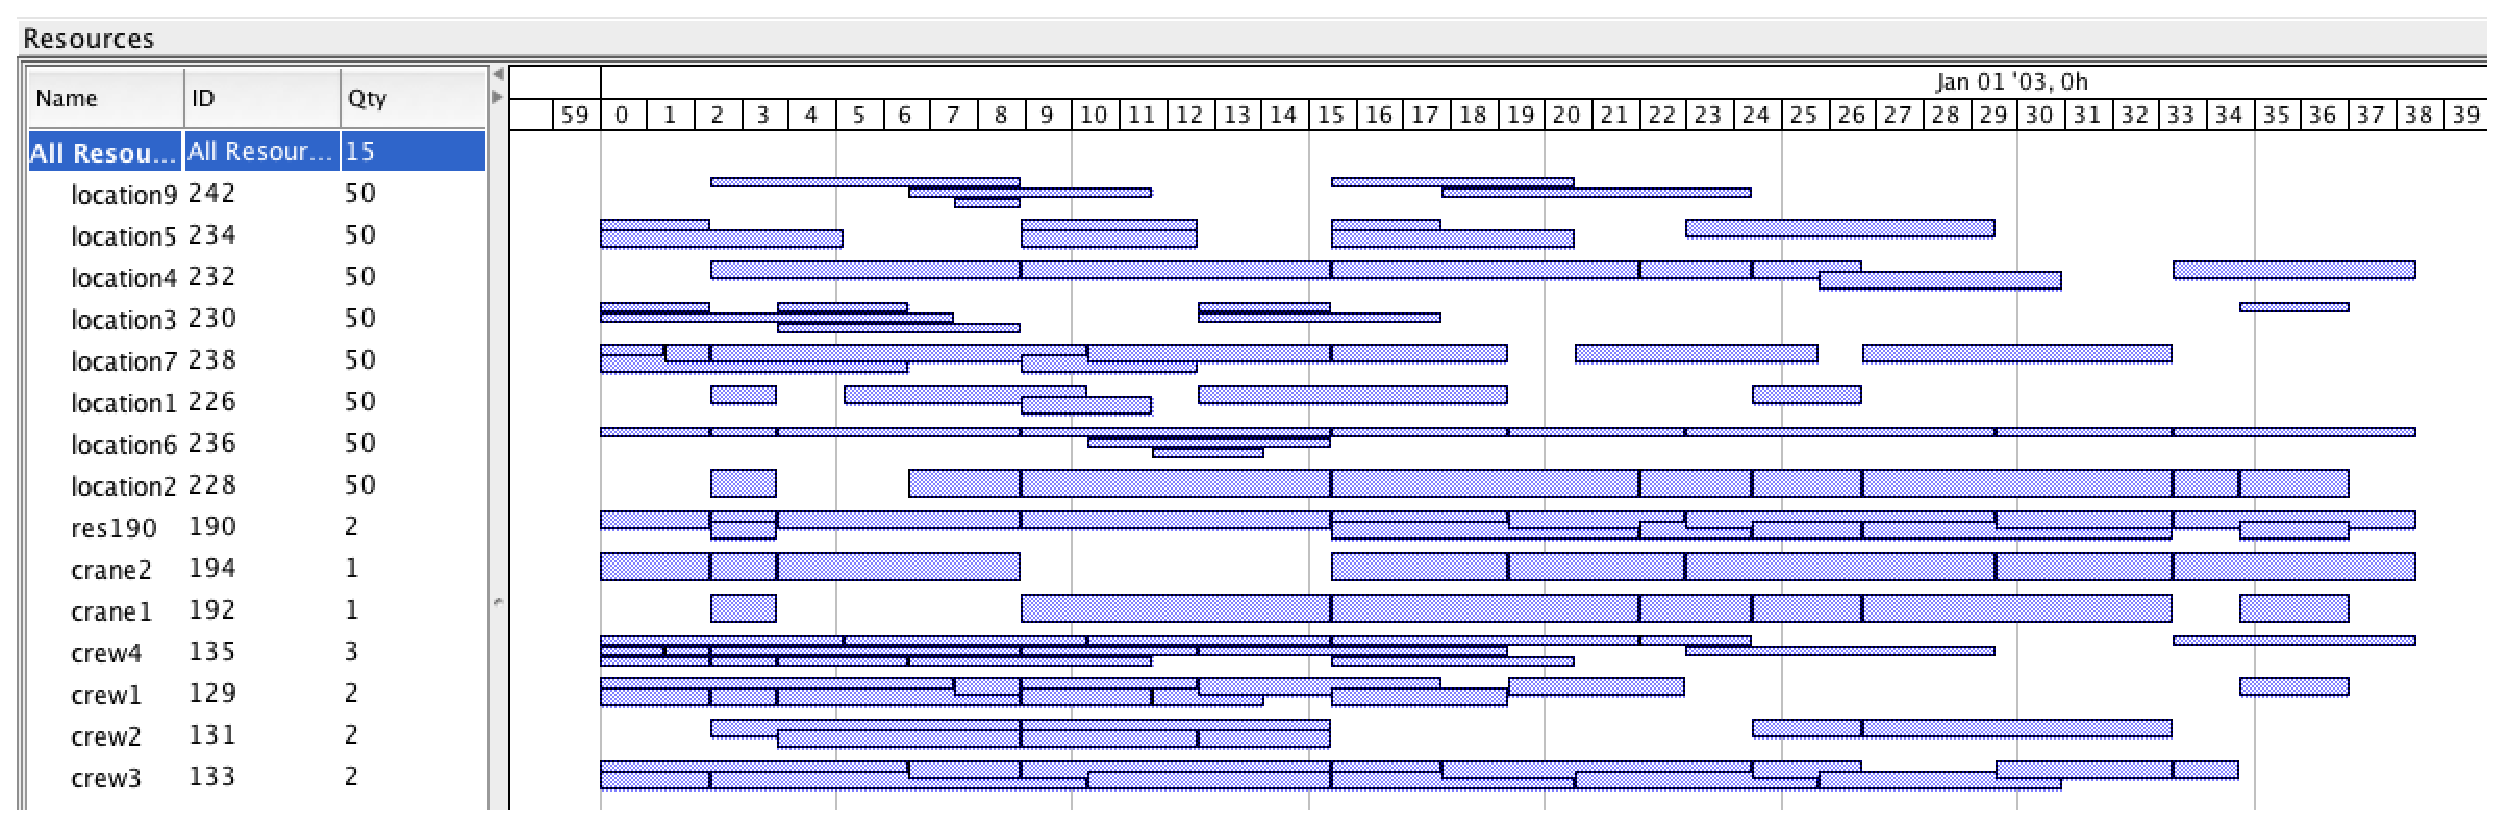
\includegraphics[scale=0.4]{content/gfx/ResourceAct50Crane2LS2_UtenVarme_100s}
\caption{Ressursskjema på Act50Loc10Crew5Crane2, LS2 og $\sharp1\sharp3$}
\label{fig:ResourceAct50Crane2LS2_UtenVarme_100s}
\end{figure}

\subsection{Med varmebegrensning}
I tabell \ref{tab:resultaterSum100s} og \ref{tab:resultaterSum5s} er dette benevnt LS1 og 2 $\sharp 2\sharp 3$ (dvs. med sikkerhetsbegrensing).

LS1 løser alle probleminstanser og har en gjennomsnittlig makespan på 81.0\%. Makespan er for alle $Act(P)$ høye - i intervallet 67.2\%-96.1\%. Figur \ref{fig:RessursWithAct50Loc10Crew5Crane2LS1} viser at for dette tilfellet er lokasjon 2 fullt utnyttet. Kran 1 er på lokasjon 2 (fra probleminstansene). Det er to kraner. Figur \ref{fig:RessursWithAct50Loc10Crew5Crane3LS1} viser at for det viste tilfellet er mannskap fullt utnyttet. Det er 3 kraner. Figur \ref{fig:GantWithAct50Loc10Crew5Crane2AssignHeat} med resultat for det viste tilfellet er vist som eksempel. Diagramet viser mange aktiviteter tidlig i planleggingen og få aktiviteter mot slutten. Tidsaksen viser en makespan på 57. Ved å benytte søketid på 5 sekunder løser LS1 94\% av probleminstansene og har en gjennomsnittlig makespan på 80.8\%. Makespan for alle $Act(P)$ høye - i intervallet 67.4\%-96.3\%.

LS2 løser i gjennomsnitt 40\% av probleminstansene og har makespan på 23.2\%. Makespan for alle $Act(P)$ er lave - i intervallet 4.1\%-31.3\%. Det laveste resultatet er for 3 kraner og $\ge 100(55)$. Figur \ref{fig:GantWithAct50Loc10Crew5Crane2TFHeat} med resultat for det viste tilfellet vises som eksempel. Diagrammet viser noe bedre fordeling av aktiviteter enn figur \ref{fig:GantWithAct50Loc10Crew5Crane2AssignHeat}. Tidsaksen viser en makespan på 48. Ved å benytte søketid på 5 sekunder løser LS2 37\% av probleminstansene med en gjennomsnittlig makespan på 22.1\%. Makespan for alle $Act(P)$ er lave - i intervallet 4.6\%-38.5\%.
\begin{figure}[!h]
\centering
\includegraphics[scale=0.25]{content/gfx/Act50Crane2GantAssignHeat}
\caption{Gantskjema på Act50Loc10Crew5Crane2 med varmebegrensning, LS1 og $\sharp2\sharp3$}
\label{fig:GantWithAct50Loc10Crew5Crane2AssignHeat}
\end{figure}
\begin{figure}[!h]
\centering
\includegraphics[scale=0.25]{content/gfx/Act50Crane2TimesForwardHeat}
\caption{Gantskjema på Act50Loc10Crew5Crane2 med varmebegrensning, LS2 og $\sharp2\sharp3$}
\label{fig:GantWithAct50Loc10Crew5Crane2TFHeat}
\end{figure}

Løsningene fra tabell \ref{tab:resultaterSum5s} med LS1 og LS2 uten sikkerhetsbegrensinger er identiske. Like mange probleminstanser er løst og gjennomsnittlig makespan verdi er også lik.

Tidene som Scheduler bruker for å finne løsninger på probleminstansene er sammenliggnet med å se på tidene for samme antall aktiviteter og henholdsvis to og tre kraner. Det er ingen klare skiller om probleminstansene inneholder to eller tre kraner. Tidene for å finne løsninger varierer fra 0 til over 100 sekunder, og det er ikke de probleminstansene med flest aktiviteter som bruker lengst tid. Tiden for å finne en løsning varierer også stort innenfor probleminstansene med samme antall aktiviteter.
%\newpage

\section{Evaluering}
I denne delen blir probleminstanser, løsningsstrategier og løsninger evaluert. Denne delen blir avsluttet med å evaluere løsningene funnet i dette prosjektet opp mot løsningene funnet i artikkelen til Bård Henning Tvedt.

Generelle forutsetninger for probleminstansene er:
Med 10 lokasjoner vil vil det i snitt være 5-500 aktiviteter pr. lokasjon. Varmekapasitet er en gitt verdi på hver lokasjon. Det er å forvente at:
\begin{itemize}
\item jo flere aktiviteter, desto større blir effekten av varmekapasiteten på lokasjonen.
\item jo høyere aktivitet (større behov for kran), desto større begrensende effekt vil kranressursene få.
\end{itemize}

\subsection{Probleminstanser}
Probleminstansene har fra 50-5000 aktiviteter, mens antall lokasjoner og mannskaper i de genererte probleminstansene er henholdsvis 10 og 5.

Det ble først eksperimentert litt med mannskapets varme og lokasjoners varmekapsitet og i det første settet med probleminstanser var det overlapp mellom mannskapers varme og en lokasjons varmekapasitet. Dette førte til veldig få løsninger når varmebegrensningen ble tatt med. Det ble funnet løsninger på noen av probleminstansene under 100 aktiviteter, mens over 100 aktiviteter var det kun en løsning. Det er grunn til å tro dette var tilfeldig, ut i fra at varme og varmekapasitet blir tilfeldig plassert innenfor et gitt område. Erfaringene fra dette er kun tatt til etterretning og resultatene er ikke interessante her pga. få løsninger.

Probleminstansene hvor varme og varmekapasitet ikke er overlappende, ga flere løsninger og er brukt videre gjennom prosjektoppgaven.

\subsection{Løsningsstrategier}
Tabell \ref{tab:resultaterSum100s} viser et ganske klart bilde av de sterke og svake sidene til de to løsningsstrategiene som er brukt. LS1 løser alle probleminstanser, mens LS2 gir betydelig bedre makespan.

Ser vi samtidig på ressursskjemaene for $LS1\sharp1\sharp3$, figur \ref{fig:RessursWithoutAct50Loc10Crew5Crane2LS1}, og $LS2\sharp1\sharp3$, figur \ref{fig:ResourceAct50Crane2LS2_UtenVarme_100s}, for gitte tilfeller, ser vi følgende:
\begin{itemize}
\item $LS1\sharp1\sharp3$ har få aktiviteter mot enden av tidsaksen. Det er lengere makespan.
\item $LS2\sharp1\sharp3$ har jevnt med aktiviteter langs tidsaksen. Det er kortere makespan.
\end{itemize}
I henhold til tidligere skisserte forventninger har dette mest sannsynlig sin årsak i at LS1 produserer flere løsninger fordi kraner med sine begrensninger er på plass tidlig i søkeprosessen.
LS2 produserer bedre løsninger fordi det tildeles startverdier til aktiviteter uten å betrakte kranfordelingen så nøye. Men antallet løsninger blir gjerne redusert fordi søkeprosessen ikke klarer å komme ut av konfliktene som oppstår når man tildeler kran senere.

Modellene uten sikkerhetsbegrensinger ga identiske løsninger. Dette er muligens fordi når sikkerhetsbegrensning på kran fjernes fungerer LS1 og LS2 likt.

\subsection{Resultater}
I denne prosjektoppgaven er en eksisterende løsning utvidet med en ressurs kalt varmeressurs. For å evaluere resultatene fra den utvidete løsningen, evalueres den utvidete løsningen med 10 lokasjoner opp mot den opprinnelige løsningen med 25 lokasjoner. Hensikten med å sammenligne resultatene fra den opprinnelige løsningen med 25 lokasjoner og 10 lokasjoner er å analysere effekten av antall lokasjoner.

Evalueringen innebærer også å analysere effekten av varmebegrensningen, som er gjort ved å sammenligne resultatene med 10 lokasjoner med og uten varmebegrensning. Evalueringen av resultatene baserer seg på gjennomsnittsverdiene i tabell \ref{tab:resultaterSum100s} og \ref{tab:resultaterSum5s}.

\subsubsection{10 Lokasjoner}
Løsningene er i ganske god overensstemmelse med forventningene i kapitel \ref{sec:implprocess}. Med LS1 hvor kranfordelingen ble valgt først var gjennomsnittlig makespan dårligere enn med LS2.

\begin{figure}[!h]
\centering
\includegraphics[scale=0.3]{content/gfx/Act50Crane2AssignHeatResourceCrane}
\caption{Ressursoversikt på Act50Loc10Crew5Crane2 med varmebegrensning, LS1, $\sharp2\sharp3$}
\label{fig:RessursWithAct50Loc10Crew5Crane2LS1}
\end{figure}
\begin{figure}[!h]
\centering
\includegraphics[scale=0.3]{content/gfx/Act50Crane2WithoutResourceCrane}
\caption{Ressursoversikt på Act50Loc10Crew5Crane2 uten varmebegrensning, LS1, $\sharp1\sharp3$}
\label{fig:RessursWithoutAct50Loc10Crew5Crane2LS1}
\end{figure}
\begin{figure}[!h]
\centering
\includegraphics[scale=0.3]{content/gfx/Act50Crane3AssignHeatResourceCrew}
\caption{Ressursoversikt på Act50Loc10Crew5Crane3 med varmebegrensning, LS1 og $\sharp2\sharp3$}
\label{fig:RessursWithAct50Loc10Crew5Crane3LS1}
\end{figure}
\begin{figure}[!h]
\centering
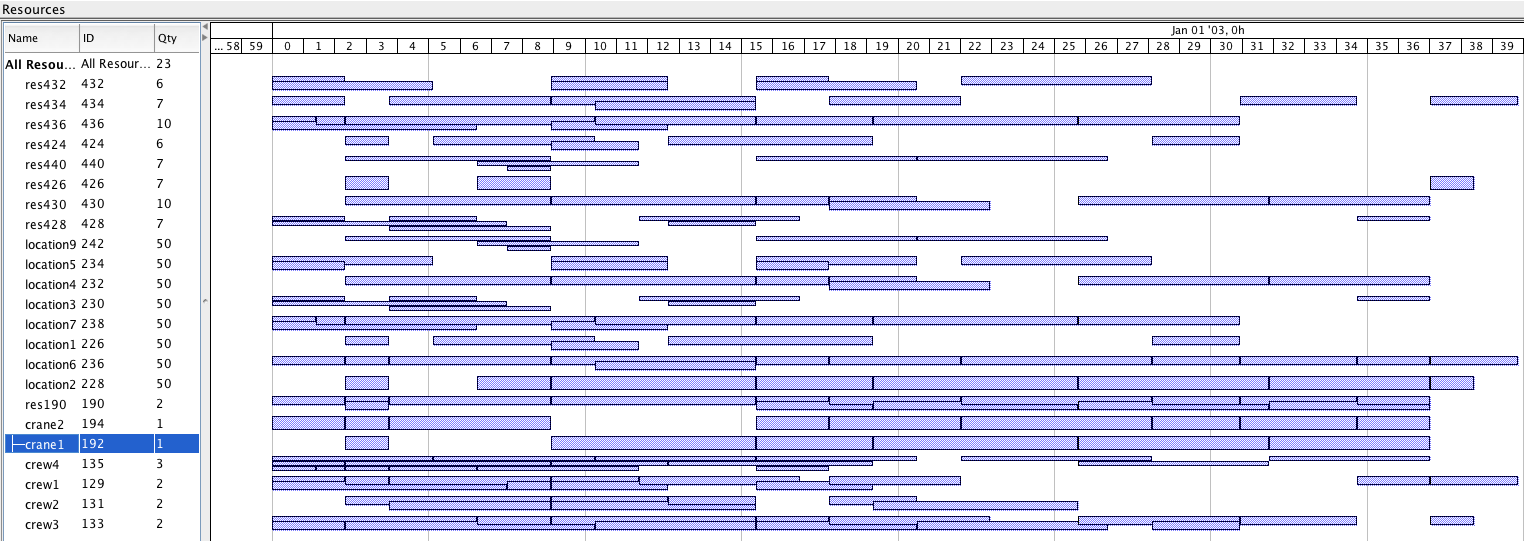
\includegraphics[scale=0.3]{content/gfx/Act50Crane2LS2WithHeat}
\caption{Ressursoversikt på Act50Loc10Crew5Crane2 med varmebegrensning, LS2 og $\sharp2\sharp3$}
\label{fig:RessursWithAct50Loc10Crew5Crane2LS2}
\end{figure}
Figur \ref{fig:RessursWithAct50Loc10Crew5Crane2LS1} og \ref{fig:RessursWithAct50Loc10Crew5Crane3LS1} er ressursdiagrammer med varmebegrensing. Til venstre i disse bildene er ressursene listet opp. De 8 øverst i denne listen er varmeressursene. Deretter følger lokasjons- og kranressursene, hvor det også er 8 lokasjonsressurser. I og med at varmeressursen er knyttet til lokasjon, er det samme antall varmeressurser som lokasjonsressurser. I og med at varmebegrensningen er knyttet til en aktivitet og lokasjonene er knyttet til en aktivitet, er det aktiviteter i disse figurene som har samme varighet under varmebegrensningen og på lokasjonsressursen. Dette er tydelig til høyre på figurene hvor det ikke er så mange aktiviteter.

Figur \ref{fig:RessursWithoutAct50Loc10Crew5Crane2LS1} er en gitt situasjon uten varmebegrensning og figur \ref{fig:RessursWithAct50Loc10Crew5Crane2LS1} er den samme med varmebegrensning. Begge figurene har lokasjon 2 fullt utnyttet. Kran 1 er på lokasjonen og er den reelle begrensningen. Innføring av varmebegrensningen gir i dette tilfellet med kran som begrensning lite utslag i henhold til tabell \ref{tab:resultaterSum100s} (liten økning i makespan). Generelt er det forventet en økning i makespan når varmebegrensing innføres. Denne økningen antas ikke i sin helhet å kun komme fra varmebegrensningen, men sannsynligvis også være et resultat at det blir vanskeligere å løse problemet.

Figur \ref{fig:RessursWithAct50Loc10Crew5Crane3LS1} kontra figur \ref{fig:RessursWithoutAct50Loc10Crew5Crane2LS1} er en gitt situasjon og økning fra to til tre kraner. Det er samme betrakning rundt utnyttelse, men i figur \ref{fig:RessursWithAct50Loc10Crew5Crane3LS1} endres dette. Her er det nå mannskap som over tid bruker hele kapasiteten.

\begin{equation}
c_{load}(Crane_{k}) = \sum_{c_{Crane}(Act_{i})=Crane_{k}} c_{dur}(Act_{i})
\label{eq:kranstyrke}
\end{equation}
Ved å sammenligne om verdier fra (\ref{eq:kranstyrke}) er mindre eller større enn (\ref{eq:mannskapsstyrke}), gir det et uttrykk for hvor sterk eller svak kranressursen er. Hvis (\ref{eq:kranstyrke}) er mindre vil det si at kranressursen er svak. Ut ifra dette er det en signifikant forskjell på to og tre kraner med LS1. Ved to kraner er kranressursen veldig sterk på kran 1, mens kranressursen ikke er fullt så sterke med tre kraner. Figur \ref{fig:RessursWithAct50Loc10Crew5Crane2LS1} viser den skjeve fordelingen mellom kran 1 og kran 2. Denne figuren viser tydelig at kran 1 er ganske godt utnyttet, mens kran 2 er mindre utnyttet. De tre aktivitetene som er helt til høyre i figur \ref{fig:RessursWithAct50Loc10Crew5Crane2LS1} krever alle kran og er tildelt kran 1. Med LS2 er det en jevnere kranfordeling som også vises i figur \ref{fig:RessursWithAct50Loc10Crew5Crane2LS2}. Med en jevnere utnyttelse av kranene som i LS2 vil også makespan kunne bli bedre. Fra resultatene og målingene gjort med (\ref{eq:kranstyrke}) opp mot (\ref{eq:mannskapsstyrke}) og ved å studere figur \ref{fig:RessursWithAct50Loc10Crew5Crane2LS1} og \ref{fig:RessursWithAct50Loc10Crew5Crane2LS2}, virker det som å tildele kraner først i søkemålet i Solver så klarer man ikke å utnytte alle kranressursene som er tilgjengelig. Men når starttidene til aktivitetene blir tildelt først virker det som tildelingen av kraner klarer å utnytte kranressursene som er tilgjengelige på en bedre måte. En mulig forklaring kan være at ved å tildele kraner først, så vil søkerommet fortsatt være såpass stort at Solver ikke finner andre mulige kraner. Det er mulig at søkerommet ved å tildele starttider til aktiviteter først vil gjøre søkerommet mindre, så det å tildele kraner etter tildeling av starttider gjør Solver i stand til å finne beste mulige kranen til aktiviteter som krever det.

Det ble tidligere fremsatt forventninger til varmebegrensningen og kraners effekt på løsningene når antall aktiviteter øker. Dette ser i all hovedsak ut til å stemme ut ifra resultatene som fremkommer i tabell \ref{tab:resultaterSum100s} og \ref{tab:resultaterSum5s}. At det er noen unntak, kan sannsynligvis forklares ved lav løsningsprosent, slik at optimale løsninger ikke kan etableres.

Tiden det tar å løse probleminstansene er også veldig lik uten noe spesielt mønster både med og uten varmebegrensning. Det er derfor litt bedre løsninger uten varmebegrensning.

Ved å ta utgangspunkt i LS2 uten varmebegrensing og uten sikkerhetsbegrensning på kran fra tabell \ref{tab:resultaterSum100s} er makespan totalt sett 1.0\% over teoretisk nedregrense med tidsgrense på 100 sekunder. Det er også løsninger på alle probleminstanser. Denne løsningen er veldig lite begrenset, da det ikke er noen grense for hvor mange mannskaper som kan være på en lokasjon og heller ingen begrensning på gjennomføring av aktiviteter ved kranbruk. Når sikkerhetsbegrensningene blir lagt til øker makespan med 13.2\% og det er ikke løsninger på mer enn 36.88\% av probleminstansene. Dette virker fornuftig med tanke på at sikkerhetsbegrensningene vil opprette sikkerhetssoner som vil stenge lokasjonen til kranen og stenger lokasjonen aktiviteten som bruker kranen blir utført på. Ytterligere øker makespan med 9\% og det blir funnet løsninger på 40\% av probleminstansene da varmebegrensningen blir lagt til. Dette viser at det kan være en tendens at innføringen av varmebegrensningen bidrar til at Scheduler finner flere løsninger. Ved å se på tabell \ref{tab:resultaterSum5s} kan det se ut som tendensen også er gjeldene med en søketid på 5 sekunder. Her er løsningsprosentene for henholdsvis LS2$\sharp 1\sharp3$ og LS2$\sharp 2\sharp3$ 36\% og 37\%. Når varmebegrensningen blir lagt til, begrenses antall mannskaper som kan jobbe på lokasjonene samtidig. Det kan se ut som Scheduler sliter med sikkerhetsbegrensningene på kran.

\subsubsection{10 lokasjoner mot 25 lokasjoner}
For å sammenligne løsningene i denne prosjektoppgaven med 10 lokasjoner, mot løsningene til \bht med 25 lokasjoner, er tabell \ref{tab:resultaterSumTvedt} hentet fra \cite{tvedtbezem}. Det benyttes henholdsvis $LS2\sharp1\sharp3$ og Inferred i sammenlikningen.
\begin{table}[!h]
\caption{Relativ optimalitets indeks $w_{rq}$ for de forskjellige modellene}
\begin{center}
\begin{tabular}{ | c | c | c | c | c | c | c | c | c | c | c | }
\hline
\textbf{Modell} & \multicolumn{4}{|c|}{\textbf{2 kraner}} & \multicolumn{4}{|c|}{\textbf{3 kraner}} & \multicolumn{2}{|c|}{\textbf{Alle}} \\ \hline
$\sharp Act(\sharp P)$ & \multicolumn{2}{|c|}{$< 100 (25)$} & \multicolumn{2}{|c|}{$> 100 (23)$} & \multicolumn{2}{|c|}{$< 100 (28)$} & \multicolumn{2}{|c|}{$> 100 (23)$} & \multicolumn{2}{|c|}{(99)} \\ 
\hline
Modell & $w_{rq}$ & $\%^{(2)}$ & $w_{rq}$ & $\%^{(2)}$  & $w_{rq}$ & $\%^{(2)}$ & $w_{rq}$ & $\%^{(2)}$ & $w_{rq}$ & $\%^{(2)}$ \\ \hline
Greedy & 1.311 & 100 & 1.524 & 100 & 1.276 & 100 & 1.393 & 100 & 1.370 & 100 \\
Inferred & 1.068 & 100 & 1.063 & 35 & 1.017 & 32 & 1.000 & 4 & 1.055 & 43 \\
Under$^{(1)}$ & 1.032 & 100 & 1.014 & 100 & 1.015 & 100 & 1.002 & 96 & 1.016 & 99 \\
Over$\sharp 1$ & 1.143 & 100 & 1.076 & 100 & 1.176 & 100 & 1.037 & 91 & 1.114 & 98 \\
Over$\sharp 2$ & 1.104 & 100 & 1.047 & 96 & 1.068 & 96 & 1.005 & 65 & 1.063 & 90 \\
\hline
\multicolumn{11}{l}{\begin{minipage}{6in}$^{(1)}$ Denne modellen garanterer ikke gyldige løsninger.
$^{(2)}$ prosentandel løste instanser \end{minipage}}
\end{tabular}
\end{center}
\label{tab:resultaterSumTvedt}
\end{table}
Det er stort samsvar mellom både makespan og løsningsgrad. Makespan er bra og varierer lite. Løsningsgrad reduseres svært mye med mange aktiviteter, både for to og tre kraner. I begge modellene tildeles tid til aktiviteter før kranressurser. Som tidligere også beskrevet om LS2 antas tendensen å skyldes at kranressurser skal tildeles i et økende antall allerede disponerte aktiviteter. I Inferred modellen i tabell \ref{tab:resultaterSumTvedt} er makespan litt bedre enn i LS2$\sharp1\sharp3$ i tabell \ref{tab:resultaterSum100s}. Dette kan muligens forklares med reduksjonen av antall lokasjoner fra 25 i tabell \ref{tab:resultaterSumTvedt} til 10 i tabell \ref{tab:resultaterSum100s}. Det blir brukt samme antall kraner, 2 og 3, som med sikkerhetssonene aktivert vil låse en mye større andel av lokasjonene i løsningene med 10 lokasjoner enn løsningene med 25 lokasjoner. Med henholdsvis 2 kraner i bruk og aktiviteter som ikke utføres på samme lokasjon som kranen befinner seg, vil det da med sikkerhetssoner bli låst 4 lokasjoner. I løsningene med 10 lokasjoner vil da 40\% av lokasjonene være låst, mens med 25 lokasjoner vil bare 16\% av lokasjonene være låst pga. sikkerhetssonene.

%Future work
\section{Fremtidig arbeid}

\begin{itemize}
\item Erstatte sikkerhetsbegrensinger med varmebegrensning
\item Innføre varmebegrensning også på kranressurser
\item Utvikle egne målsetninger i Solver.
\end{itemize}
%\newpage

%Conclusion
\section{Konklusjon}
Målet med denne masteroppgaven var å se på utfordringer innen automatisk vedlikeholdsplanlegging i oljeindustrien. Det er prøvd ut forskjellige løsningsstrategier samt lagt til en varmebegrensning. Alt for å ta hånd om vedlikeholdsplanlegging i olje og gassindustrien som har høye krav høye krav til planlegging, kvalitetssikring og gjennomføring.

Den første løsningsstrategien (LS1), som tildelte kraner først, løste alle probleminstansene uavhengig av størrelse og kompleksitet. For implementasjonen uten varmebegrensing og deretter med varmebegrensning ligger løsningene henholdsvis 74.5\% og 81.0\% over teoretisk nedregrense. 

Den andre løsningsstrategien (LS2), som tildeler starttidspunkt til alle aktivitene først, løste ikke alle probleminstansene, men har de beste løsningene i forhold til teoretisk nedregrense. For implementasjonen uten varmebegrensning og deretter med varmebegrensning ligger løsningene henholdsvis 14.2\% og 23.2\% over teoretisk nedregrense.

Det kan være hensiksmessig å vurdere hvilken løsningsstrategi som skal brukes avhengig av om det er ønskelig med å ha høy løsningsgrad eller bedre makespan.

Løsningene med varmebegrensning ga med begge løsningsstrategiene noe høyere makespan enn uten varmebegrensning. Dette kan være både en reell økning av nedre grense eller være en økning av at problemet er mer komplekst å løse, eller en kombinasjon av begge. Resultatene viser at løsningsstrategien har større betydning enn varmebegrensningen når det gjelder hvor mange probleminstanser som blir løst. Det ser ut som det å legge til varmebegrensing ikke forbedrer makespan og det må tas beslutninger på om det er best mulig løsninger eller flest mulig løsninger som er ønskelig når det skal utvikles en appliksjon med Scheduler.
\newpage

%Appendix
\section{Vedlegg}
\begin{center}								
\begin{table}[h]								
\begin{tabular}{ | l | c | c | c |}								
\hline								
Benchmark &	Teoretisk nedregrense  	& Teoretisk øvregrense bound &	Makespan \\	\hline
Act1000Loc10Crew5Crane2\_1 & 416	& 3529 & 449	\\
Act100Loc10Crew5Crane2\_1 &	50	&	356	&	50	\\	
Act100Loc10Crew5Crane2\_2 &	66	&	364	&	67	\\	
Act100Loc10Crew5Crane2\_3 &	55	&	352	&	56	\\	
Act200Loc10Crew5Crane2\_1 &	92	&	711	&	104	\\	
Act200Loc10Crew5Crane2\_2 &	124	&	742	&	124	\\	
Act200Loc10Crew5Crane2\_3 &	66	&	704	&	89	\\	
Act200Loc10Crew5Crane2\_4 &	71	&	734	&	109	\\	
Act200Loc10Crew5Crane2\_5 &	88	&	698	&	93	\\	
Act300Loc10Crew5Crane2\_1 &	144	&	1049	&	144	\\	
Act300Loc10Crew5Crane2\_4 &	137	&	1071	&	148	\\	
Act400Loc10Crew5Crane2\_1 &	177	&	1400	&	192	\\	
Act400Loc10Crew5Crane2\_3 &	198	&	1369	&	198	\\	
Act400Loc10Crew5Crane2\_4 &	168	&	1362	&	187	\\	
Act400Loc10Crew5Crane2\_5 &	136	&	1361	&	190	\\	
Act500Loc10Crew5Crane2\_2 &	234	&	1723	&	257	\\	
Act500Loc10Crew5Crane2\_4 &	212	&	1798	&	243	\\	
Act600Loc10Crew5Crane2\_2 &	282	&	2201	&	297	\\	
Act500Loc25Crew5Crane2\_5 &	223	&	1708	&	223	\\	
Act50Loc10Crew5Crane2\_1 & 28	&	177	&	34	\\	
Act50Loc10Crew5Crane2\_4 & 21	&	172	&	22	\\	
Act50Loc10Crew5Crane2\_5 & 22	&	177	&	27	\\	
Act60Loc10Crew5Crane2\_1 & 29	&	211	&	35	\\	
Act60Loc10Crew5Crane2\_2 & 31	&	215	&	39	\\	
Act60Loc10Crew5Crane2\_3 & 31	&	209	&	38	\\	
Act60Loc10Crew5Crane2\_4 & 27	&	203	&	27	\\	
Act60Loc10Crew5Crane2\_5 & 27	&	205	&	46	\\	
\hline								
\end{tabular}								
\caption{Løsninger uten tilleggsressurser og tidsgrense på 10 sekunder}								
\label{tab:without10}								
\end{table}								
\end{center}

\begin{center}
\begin{table}[h]
\begin{tabular}{ | l | c | c | c | }
\hline
Benchmark &	Teoretisk nedregrense & Teoretisk øvregrense &	Makespan \\ \hline
Act500Loc25Crew5Crane2\_5 & 223	& 1708 & 223	\\
Act50Loc10Crew5Crane2\_1	& 28 &	177	& 34	\\
Act50Loc10Crew5Crane2\_4	& 21 &	172	& 23	\\
Act50Loc10Crew5Crane2\_5	& 22 &	177	& 29	\\
Act60Loc10Crew5Crane2\_1	& 29 &	211	& 32	\\
Act60Loc10Crew5Crane2\_2	& 31 &	215	& 41	\\
Act60Loc10Crew5Crane2\_3	& 31 &	209	& 36	\\
Act60Loc10Crew5Crane2\_4	& 27 &	203	& 27	\\
Act60Loc10Crew5Crane2\_5	& 27 &	205	& 46	\\
\hline
\end{tabular}
\caption{Løsninger med tilleggsressurser og tidsgrense på 10 sekunder}
\label{tab:with10}
\end{table}
\end{center}
\newpage

%References
\bibliography{ref}
\bibliographystyle{plain}

% END OF DOCUMENT
\end{document}